\documentclass{projetofinal-dcc}
%%%%%%%%%%%%%%%%%%%%%%%%%%%%%%%%%%%%%%%%%%%%%%%%%%%%%%%%%%%%
%P A C O T E S
%%%%%%%%%%%%%%%%%%%%%%%%%%%%%%%%%%%%%%%%%%%%%%%%%%%%%%%%%%%%
% Adicione aqui seus pacotes
\usepackage[version = 2]{acro}
\usepackage[]{algorithm2e}
\usepackage{paralist}
\usepackage{float}
\usepackage{verbatim} % para comments
\usepackage{mathtools} % para fórmulas matemáticas
%%%%%%%%%%%%%%%%%%%%%%%%%%%%%%%%%%%%%%%%%%%%%%%%%%%%%%%%%%%%
%I N I C I O  D O  D O C U M E N T O
%%%%%%%%%%%%%%%%%%%%%%%%%%%%%%%%%%%%%%%%%%%%%%%%%%%%%%%%%%%%
\begin{document}

\definecolor{dkgreen}{rgb}{0,0.6,0}
\definecolor{gray}{rgb}{0.5,0.5,0.5}
\definecolor{black}{rgb}{0,0,0}
\definecolor{blue}{rgb}{0,0,0.4}
\definecolor{purple}{rgb}{0.8,0,0.3}
\definecolor{orange}{rgb}{1,0.4,0}
\definecolor{lightlightgray}{gray}{0.85}

% título da tese é obrigatório
\title{Avaliação da Adição de Captions na Detecção de
Anomalia}

% autor é obrigatório; máximo de 3 autores
\author{Bárbara Lúcia Martins Barboza}{Aos Deuses e a Alá!}
%\author{Nome completo aluno 2}{Aos Deuses e a Alá!}
%\author{Nome completo aluno 3}{Aos Deuses e a Alá!}

% orientador é obrigatório
\advisor[Prof.]{Leandro Guimarães M. Alvim,~D.Sc.}{}
% \advisor[Prof.]{Nome completo,~D.Sc.}{}{a} % orientadora

% co-orientador é opcional
%\coadvisor[Prof.]{Nome do co-orientador,~M.Sc.}{}
%\coadvisor[Prof.]{Nome do co-orientador,~M.Sc.}{}{a} % co-orientadora

% máximo de 3 integrantes da banca (orientador e co-orientador já são adicionados automaticamente)
\banca[Prof.]{Nome do participante banca 1,~D.Sc.}{DCC~-~UFRRJ}
\banca[Prof.]{Nome do participante banca 2,~Ph.D.}{DCC~-~UFRRJ}
%\banca[Prof.]{Nome do participante banca 3,~Ph.D.}{DCC~-~UFRRJ}

\location{Nova Iguaçu}{RJ}{Brasil}

% mês e ano de defesa
\date{Julho}{2023}
\maketitle

\startdocument
%%%%%%%%%%%%%%%%%%%%%%%%%%%%%%%%%%%%%%%%%%%%%%%%%%%%%%%%%%%%
%A G R A D E C I M E N T O S
%%%%%%%%%%%%%%%%%%%%%%%%%%%%%%%%%%%%%%%%%%%%%%%%%%%%%%%%%%%% 
\makethankspage

%%%%%%%%%%%%%%%%%%%%%%%%%%%%%%%%%%%%%%%%%%%%%%%%%%%%%%%%%%%%
%R E S U M O
%%%%%%%%%%%%%%%%%%%%%%%%%%%%%%%%%%%%%%%%%%%%%%%%%%%%%%%%%%%%
\begin{abstract}{
  Cada vez mais tem crescido o número de câmeras de segurança presentes nas cidades, não só em locais públicos, mas até a nível pessoal, muitas vezes possuímos câmeras em nossas casas. Elas são usadas para que tenhamos mais seurança e para que, no caso de algum incidente, as atitudes cabíveis possam ser tomadas o mais rápido possível. Porém, com esse aumento do número de câmeras, torna-se humanamente impossível ficar observando as imagens para tomar ciência de qualquer incidente que possa ter ocorrido. É nesse contexto que a tecnologia pode ajudar, através de algoritmos de \textit{Machine Learning} é possível que os eventos anômalos sejam detectados automaticamente. 

Estudos sobre detecção de anomalia utilizando as imagens capturadas pelas câmeras já vem sendo feitos há alguns anos, geralmente utilizando redes neurais convolucionais. O objetivo desse trabalho no entanto, é adicionar \textit{captions}, ou seja, descrições das imagens, além das imagens em si, e verificar se há algum ganho expressivo no acerto do algoritmo utilizando as \textit{captions}.

%Essa parte será o resumo do trabalho em poucas frases. Nessa parte deverá conter uma explicação sobre o problema e a proposta, finalizando em como ela se comportou com relação as demais soluções da literatura.
}
\end{abstract}

%%%%%%%%%%%%%%%%%%%%%%%%%%%%%%%%%%%%%%%%%%%%%%%%%%%%%%%%%%%%
%A B S T R A C T
%%%%%%%%%%%%%%%%%%%%%%%%%%%%%%%%%%%%%%%%%%%%%%%%%%%%%%%%%%%%
\begin{englishabstract}{
  The number of security cameras in cities has been increasing, not only in public places, but even on a personal level, many times we have cameras in our homes. They are used so that we feel more safe and so that, in the case of an incident, the appropriate actions can be taken as quickly as possible. However, with this increase in the number of cameras, it becomes humanly impossible to keep watching the images to become aware of any incident that may have occurred. It is in this context that technology can help, through \textit{Machine Learning} algorithms it is possible that anomalous events are detected automatically.

Studies about anomaly detection using images captured by cameras have been done for some years, usually using convolutional neural networks. The goal of this work, however, is to add \textit{captions}, that is, images descriptions, in addition to the images themselves, and to verify if there is any expressive gain in the algorithm's accuracy using the \textit{captions}.





%Cada vez mais tem crescido o número de câmeras de segurança presentes nas cidades, não só em locais públicos, mas até a nível pessoal, muitas vezes possuímos câmeras em nossas casas. Elas são usadas para que tenhamos mais seurança e para que, no caso de algum incidente, as atitudes cabíveis possam ser tomadas o mais rápido possível. Porém, com esse aumento do número de câmeras, torna-se humanamente impossível ficar observando as imagens para tomar ciência de qualquer incidente que possa ter ocorrido. É nesse contexto que a tecnologia pode ajudar, através de algoritmos de \textit{Machine Learning} é possível que os eventos anômalos sejam detectados automaticamente. 

%Estudos sobre detecção de anomalia utilizando as imagens capturadas pelas câmeras já vem sendo feitos há alguns anos, geralmente utilizando redes neurais convolucionais. O objetivo desse trabalho no entanto, é adicionar \textit{captions}, ou seja, descrições das imagens, além das imagens em si, e verificar se há algum ganho expressivo no acerto do algoritmo utilizando as \textit{captions}.

%Será exatamente a tradução para o inglês do resumo.%
}
\end{englishabstract}

%%%%%%%%%%%%%%%%%%%%%%%%%%%%%%%%%%%%%%%%%%%%%%%%%%%%%%%%%%%%
%L I S T A S
%%%%%%%%%%%%%%%%%%%%%%%%%%%%%%%%%%%%%%%%%%%%%%%%%%%%%%%%%%%%
% Figuras
\makefigurespage

% Tabelas
\maketablespage

% Algoritmos
\makelistingspage

% Abreviaturas (devem estar em ordem alfabética)
\makeabrevpage{%%novalidate
% Abreviaturas não aparecem pq não estão senod utilizadas no texto ainda
\begin{acronym}[xxxxxxx]
    \acro{IA}{Artificial Intelligence}
    \acro{ML}{Machine Learning}
    \acro{ANN}{Artificial Neural Network}
    \acro{MLP}{Multilayer Perceptron}
    \acro{CNN}{Convolutional Neural Network}
    \acro{MAPE}{Mean Absolute Percentage Error}
    \acro{MAPD}{Mean Absolute Percentage Deviation}
\end{acronym}
% Eu já consegui!
% \begin{acronym}[xxxxxxx]
%     \acro{SR}{Sistema de Recomendação}
%     \acro{MAE}{Mean Absolute Error}
%     \acro{RMSE}{Root Mean Absolute Error}
% \end{acronym}}

% Símbolos (devem estar em ordem alfabética)
\makesymbolspage{\begin{acronym}[xxxxXXX]
    \acro{rv}[$\bar{r}_v$]{média das notas do item v}
    \acro{ru}[$\bar{r}_u$]{média das notas do usuário u}
\end{acronym}}

% Sumário 
\maketocpage

%%%%%%%%%%%%%%%%%%%%%%%%%%%%%%%%%%%%%%%%%%%%%%%%%%%%%%%%%%%%
%C O N T E Ú D O
%%%%%%%%%%%%%%%%%%%%%%%%%%%%%%%%%%%%%%%%%%%%%%%%%%%%%%%%%%%%
\startcontent
\chapter{Introdução}\label{chp:INTRODUCAO}

Com o grande aumento de sistemas de câmeras de vigilância pelas cidades, atrelado a maior capacidade computacional dos dispositivos eletrônicos, a área de visão computacional tem despertado o interesse de muitos perquisadores pelo mundo [REF]. E, quando se trata disso, uma tarefa específica da visão computacional tem grande espaço com os sistemas de vigilância: a detecção de anomalia.

Segundo o dicionário Aurélio, anomalia significa irregularidade ou anormalidade [REF]. Quando falamos em eventos anômalos, nos referimos a acontecimentos que fogem do normal ou do esperado em um determinado contexto. Um exemplo é uma câmera de vigilância numa estrada que registra diariamente veículos diversos passando pela pista. Nesse caso, esse cenário é considerado normal. Se, em algum dia, há uma batida entre dois veiculos, esse evento é considerado uma anomalia.

O interesse na detecção de anomalia reside na possibilidade de tomar as medidas necessárias imediatamente. No caso de um crime, por exemplo, assim que detectado, pode-se chamar a polícia; em caso de incêncio ou acidente, os bombeiros ou o serviço de atendimento móvel do local. Em todo caso, detectar eventos anômalos é importante para que se possa diminuir os efeitos negativos deles.

Sendo assim, pode-se imaginar que algum profissional poderia ficar analisando todas as imagens para decidir o que é ou não anomalia. Porém, esse processo seria inviável, devido à necessidade de atenção constante do(s) observador(es) a todas as imagens. Além disso, ao colocar humanos para fazerem essa tarefa, existe também a maior probabilidade de erro, dado que, o que pode ser considerado anomalia para um, pode não ser um evento anômalo para outro. Além da provável falta de percepção de alguns detalhes que poderiam ajudar a categorizar algo como anomalia ou não.

Sendo assim, a detecção manual de anomalia é inviável, sendo necessária a programação de algum sistema para fazê-la. É possível encontrar na literatura muitos textos a respeito desse assunto, alguns voltados para um contexto específico, outros para contextos mais generalizados. O fato é que muitas vezes usa-se Inteligência Artificial para essa tarefa, mais especificamente Redes Neurais Artificiais, que serão explicadas com mais detalhes mais a frente.

%Falará um breve introdução ao trabalho, explicando brevemente o contexto, motivação e problema.%

\section{Objetivos e Metodologia}

Esse trabalho tem como objetivo analisar uma possível melhora nos sistemas de detecção de anomalia tradicionais, que utilizam Redes Neurais Convolucionais, adicionando um elemento na aprendizagem: as descrições das imagens, também chamadas de \textit{captions}. Sendo assim, além da detecção de padrões nas imagens em si, haverá também a entrada de texto, e assim, um sistema mixed-input, com mais de uma entrada na Rede Neural. 

A abordagem padrão na detecção de Anomalia é utilizar um \textit{autoencoder}, ou seja, uma rede que aprenda a reconstruir a entrada fornecida, tendo assim a entrada igual a saída, com o mínimo de erro possível.

No caso desse trbalho, para observar se a adição das captions ao modelo melhoraria a detecção dos eventos anômalos, foram feitas duas arquiteturas de redes neurais: uma com camadas convolucionais e MaxPooling, e uma última camada \textit{fully Connected} para aprendizado; e a outra, uma MLP (\textit{Multilayer Perceptron}) para a parte das captions.

Foi selecionado para o trabalho um \href{https://paperswithcode.com/dataset/ubi-fights}{dataset de anomalia de brigas} em diversos ambientes. Esse dataset possui vídeos de câmeras de segurança e os targets para cada frame dos vídeos em um arquivo Excel. Dado que o problema de Detecção de Anomalia é fortemente dependente do contexto [REF], foi escolhido um vídeo de briga em uma contexto específico, e seus frames, extraídos. Assim, as imagens dos frames foram postas como a entrada da primeira arquitetura de rede neural.

Ao passo que, para a execução da segunda arquitetura, foi utilizado o pacote \href{https://github.com/OFA-Sys/OFA}{OFA} para a execução das captions das imagens. E, posteriormente, tendo as captions, foi utilizada a ferramenta de \href{https://radimrehurek.com/gensim/models/doc2vec.html}{Doc2Vec} do Gensim para transformar os textos das captions em vetores.

Então, a saída das duas redes neurais foi concatenada como a entrada para uma última camada que reconstroi as imagens dos frames dos vídeos que representam eventos não anômalos.

Além dessa execução utilizando uma MLP e uma CNN, foi feita também a abordagem padrão para resolver o problema, utilizando somente a CNN, para posterior comparação entre as duas abordagens.

E então, para as duas arquiteturas de redes, utilizando o conjunto de validação, foi calculado um limiar do erro na reconstrução das imagens que indicaria se as imagens possuíam eventos anômalos ou não. Caso o erro na reconstrução da entrada no conjunto de teste passasse desse limiar, então, o modelo estaria indicando que a imagem contém uma anomalia, se não, a imagem seria considerada normal.

Ao final desse trabalho, as predições das duas arquiteturas de redes neurais foram comparadas, chegando-se a uma conclusão sobre se houve uma melhora no modelo com a introdução das captions ou não.
%Nesta subseção seria definido os objetivos do projeto final.%

\section{Resumo dos Resultados}
Na tabela \ref{tab:RESULTADOS_MIXED_INPUT_E_CNN} temos os erros médios para imagens normais e com anomalia, os limiares e o \textit{f1 score} e acurácia para cada classe para cada modelo.

\begin{table}[!htb]
  \centering
  \label{tab:RESULTADOS_MIXED_INPUT_E_CNN}
  %\rowcolors{1}{}{lightlightgray}
  \begin{tabular}{l c c c c}
  \toprule
    & Erro Médio & Limiar & F1 Score & Acurácia \\
    \midrule
        Mixed-input &  &  &  & \\
        \hspace{0.5cm}Normal & 4 & - & 1 & 2\\
        \hspace{0.5cm}Anomalia & 4 & 3 & 3 & 1\\
        CNN &  &  &  &  \\
        \hspace{0.5cm}Normal & 4 & - & 3 & 1\\
        \hspace{0.5cm}Anomalia & 4 & $\emptyset$ & 3 & 1\\

    \bottomrule
  \end{tabular}
  \caption{Resultados do experimento CNN com caption vs somento CNN.}
\end{table}

\textit{TO DO :: TABLE WITH RESULTS}

\section{Principais Contribuições}
\begin{itemize}
  \item \textit{Estudo sobre Detecção de Anomalia}
  
  Este trabalho contribuiu como material de estudo sobre o problema de Detecção de Anomalia, escrito em língua portuguesa, utilizando ainda dados reais.
  
  \item \textit{Estudo sobre o impacto da adição de captions na detecção de anomalia}

  Essa dissertação contribuiu ainda com o estudo de uma proposta  de melhoria nos modelos de Detecção de Anomalia tradicionais, comparando a proposta com modelos apenas de CNN e verificando que os modelos tradicionais tendem a obter melhor acurácia do que modelos em que acrestamos as descrições das imagens. \textit{TO DO :: CONFIRMAR ESSE RESULTADO DE QUE A CNN ONLY É MELHOR DO QUE MIXED-INPUT}
  
\end{itemize}

\section{Organização da Dissertação}

Esse trabalho será organizado da seguinte maneira:

O capítulo 1 fez uma breve introdução ao tema, objetivo e metodologia do trabalho, além do resumo dos resultados e contribuições.

O capítulo 2 conterá uma fundamentação teórica e alguns conceitos essenciais para o entendimento do trabalho.

O capítulo 3 tratará de alguns desafios específicos do problema de Detecção de Anomalia.

O capítulo 4 apresentará a proposta em mais detalhes, bem como também os trabalhos relacionados. 

Já no capítulo 5, será apresentada a base de dados utilizada, toda a metodologia, os experimentos e resultados.

O capítulo 6 finalizará apresentando a conclusão do trabalho, assim como possíveis trabalhos futuros.

%Nesta parte, será explicada como será a organização do trabalho.%
\chapter{Fundamentação Teórica}\label{chp:FUNDAMENTACAO_TEORICA}

Esse capítulo tem como objetivo promover um esclarecimento sobre o arcabouço teórico necessário para o entendimento do trabalho. Como dito anteriormente, assim como diversos outros problemas hoje em dia, a Detecção de Anomalia é resolvida através de técnicas de aprendizado de máquina. Nesse capítulo, será tratado com mais detalhes o que é aprendizado de máquina, e algumas técnicas utilizadas para fazer com que uma máquina aprenda determinada tarefa. Posteriormente, será abordado com mais detalhes como essas técnicas são aplicadas para o contexto específico de Detecção de Anomalia e alguns desafios encontrados nessa aplicação.

% abordados alguns desafios na utilização dessas técnicas para o contexto específico de Detecção de Anomalia especificamente
% á tratado como ué possível que problema de Detecção de Anomalia é resolvido utilizando técnicas de aprendizado de máquina.  tratando-o com mais detalhes e explicando suas motivações e desafios. Será abordado o tema Aprendizado de Máquina, primordial para o entendimento do problema, e seus diversos tipos. E, por último, Redes Neurais, que geralmente é a técnica de aprendizado de máquina utiliza para a identificação de cenários anômalos.

\section{Aprendizado de Máquina}
Aprendizado de Máquina é um subcampo da Inteligência Artificial destinado a fazer máquinas aprenderem tarefas sem serem explicitamente programadas para tal. A área de Aprendizado de Máquina é inspirada por diversas outras áreas, como ciências cognitivas, ciência da computação, estatística, complexidade computacional, teoria da informação, teoria de controle, filosofia e biologia. \cite{machine_learning_yao_liu}

Segundo \citeonline{naqa_e_murphy}, um algoritmo de aprendizagem de máquina é um processo que usa dados como entrada para realizar uma tarefa desejada, sem ser literalmente programado para produzir uma saída em específico, mas se alterando e adaptando sua arquitetura através da experiência, o que é chamado de aprendizado.

Um dos pioneiros na área de Machine Learning foi Arthur Samuel. Em 1959, ele publicou um artigo dissertando sobre um algoritmo que aprendia a jogar Xadrez, afirmando que o aprendizado acontecia entre 8 e 10 horas, e que o computador era capaz de jogar melhor do que a própria pessoa que o programou. \cite{arthur_samuel_xadrez}

Posteriormente, outro grande nome da área de \ac{ML}
, Tom M. Mitchell, professor universitário, fundador e ex-presidente do Departamento de Machine Learning da Universidade
Carnegie Mellonara, definiu aprendizado de máquina da seguinte forma: \textit{"Pode-se dizer que um programa de computador aprende a partir da experiência E, a executar alguma classe de tarefas T, dada uma medida de desempenho P, quando sua performance nas tarefas em T, medida por P, melhora com a experiência E."}\cite{machine_learning_tom_mitchell}

Como dito anteriormente, o processo de aprendizagem de máquina requer dados como entrada. E nas últimas décadas, devido ao \textit{boom} dos dados, onde a quantidade de informações geradas por pessoa cresce a cada ano, essa área vem se disseminando muito rapidamente. Grande exemplo disso é o \href{https://openai.com/blog/chatgpt}{\textit{ChatGPT}}, um \textit{bot} lançado pela empresa de IA, OpenAI, em 2022, que é livre para qualquer usuário da internet testar.

% TO DO : encontrar artigo q embase a parte dos "dados gerados por pessoa crescerem muito". Só achei esse link na internet: https://uoledtech.com.br/blog/transformacao-digital-e-so-tecnologia

%comments saved

\section{Tipos de Aprendizado de Máquina}

A ciência de fazer máquinas aprenderem é dividida em três grandes tipos: aprendizado supervisionado, aprendizado não-supervisionado e aprendizado por reforço.

No aprendizado supervisionado, os dados utilizados são rotulados, isto é, além das características dos dados, tem-se também a resposta esperada que a máquina forneça para cada ocorrência do dado. Assim, a ideia é que o algoritmo vá aprendendo ao longo do treinamento as características mais importantes e os padrões gerais existentes nos dados, a fim de generalizar o suficiente para prever as respostas corretas para exemplos de dados ainda não vistos.

Nesse tipo de aprendizado, existem as tarefas de classificação e de regressão. [REF] Uma tarefa é dita de regressão, quando o rótulo dos dados é contínuo, está no conjunto dos Reais. Ao passo que, uma tarefa é dita de classificação, quando o domínio dos rótulos dos dados é um subconjunto bem definido de valores, geralmente inteiros, onde cada valor especifica uma classe.

Enquanto o aprendizado supervisionado utiliza dados rotulados, no aprendizado não supervisionado, os dados não possuem rótulos ou gabaritos. Nesse modelo, o que ocorre é uma aprendizagem heurística no decorrer do treinamento.

% falar um pouco mais sobre o não supervisionado %

Há, ainda, entre o aprendizado supervisionado e o não-supervisionado, o semi-supervisionado, que consiste numa tentativa de suprir as desvantagens de cada um dos métodos com as vantagens do outro. Nessa abordagem, o treinamento começa com os dados obtidos que possuam rótulo, a fim de adquirir algum conhecimento a respeito do problema que ajude no aprendizado com os dados não rotulados, que se segue.\cite{tcc_anomalia_2020}

Além do aprendizado com supervisão ou não, existe ainda um outro tipo de aprendizado, que começou a surgir na literatura na década de 1990, o aprendizado por reforço. No ano de 1998, \citeauthor{drive_a_bicycle_rl_jette} publicaram um artigo explicando como seria possível aprender a andar de bicicleta utilizando aprendizado por reforço. No mesmo ano, \citeauthor{rl_an_introduction} publicaram o livro \textit{Reinforcement Learning: An Introduction}, explicando mais em detalhes o aprendizado por reforço. \cite{rl_an_introduction}

Esse tipo de aprendizado se baseia fundamentalmente na interação com o ambiente, onde, a cada iteração, a máquina capta as percepções do estado do ambiente e realiza alguma ação. E essas ações são medidas como boas ou não através de uma função chamada recompensa ou penalização.

Tendo dado uma breve introdução a respeito dos diversos tipos de aprendizado de máquina, serão explicados a seguir conceitos mais específicos necessários para o entendimento do trabalho aqui proposto, bem como para o desenvolvimento da solução de Detecção de Anomalia.


% DRAFT --- DRAFT --- DRAFT 
% No aprendizado supervisionado, para medir o aprendizado, temos uma função que, de algum modo, calcula a diferença entre os rótulos esperados (reais) e os obtidos como saída do algoritmo no conjunto de teste.

% é dito que a tarefa é de regressão. Enquanto, quando o rótulo está num conjunto bem definido 
% Nesse tipo de aprendizado, para medir o aprendizado, utiliza-se uma função, f : X X Y -> R. é necessária uma medida para saber

% comments saved

% lero-lero o q aprendizado ?
% tipos de aprendizado
% supervisionado def
% supervisionado fç de custo / performance
% não supervisionaod def (exemplo)
% semi-supervisionado def
% por ref def
% por ref mais deta (agente, tempo, função)


\section{Redes Neurais Artificiais}
Um dos modelos de \ac{IA} mais famosos e que tem sido muito utilizado hoje em dia é o de Redes Neurais Artificias (\textit{Artificial Neural Networks} ou \textit{ANNs}). Isso se dá devido ao fato de que, com esse modelo, é possível o aprendizado de muitos problemas complexos, que outros modelos não são capazes de aprender. Alguns desses problemas são o reconhecimento de fala, reconhecimento facial, reconhecimento de caracter escrito a mão, classificação de imagens, detecção de objetos em imagens, entre outros.

O modelo de \ac{ANN} foi inspirado nas redes neurais biológicas existentes nos seres vivos. De forma simplória, é possível defini-lo como um conjunto de unidades simples, densamente interconectadas, onde cada unidade recebe um número de entrada real, que pode ser a saída de outras unidades, e produz um único valor de saída real, que pode se tornar a entrada de outras unidades.\cite{machine_learning_tom_mitchell, tcc_anomalia_2021}
% TO DO : how to deal with 2 references?

\subsection{Perceptron}
A forma mais simples de unidade de rede neural que existe na literatura é o \textit{perceptron}. O \textit{perceptron} foi criado por \citeauthor{perceptron_frank_rosenblatt}, psicólogo americano, em 1958, e nada mais é do que um algoritmo iterativo que produz um resultado através da
combinação linear entre os valores de entrada \(x_{1}, x_{2}, x_{3}, ..., x_{n}\) e um vetor de valores
\(w_{0}, w_{1}, w_{2}, ..., w_{n}\) que serão otimizados durante a execução.\cite{perceptron_frank_rosenblatt}\cite{tcc_anomalia_2020}
% TO DO : how to deal with 2 references?

O vetor \(\overrightarrow{w}\), chamado de vetor de pesos, é composto de valores reais, onde cada \(w_{i}\) determina a contribuição da entrada \(x_{i}\) à saída do perceptron.\cite{machine_learning_tom_mitchell} Caso o resultado da combinaçao linear entre os vetores seja maior do que 0, a saída do perceptron é 1, se não, é -1. Assim, a função \(\ \theta (x_{1}, ..., x_{n})\) computada pelo \textit{perceptron} é definida da seguinte forma:
\begin{equation}
%\[
    \theta (x_{1}, \cdots, x_{n}) = 
    \begin{cases}
         \quad1       & \quad \text{caso } w_{0} + w_{1}x_{1} + ... + w_{n}x_{n} > 0\\
        -1  & \quad \text{caso contrário}
    \end{cases}
%\]
\label{eq:eq_perceptron_extenso}
\end{equation}

Ainda, para simplificar, podemos imaginar uma entrada constante \(x_{0} = 1\). Dessa forma, temos \( \sum_{i=0}^n w_{i}x_{i} \), que também pode ser chamado de produto escalar entre \(\overrightarrow{w}\) e \(\overrightarrow{x}\). Sendo assim, a \refequation{eq:eq_perceptron_extenso} também pode ser descrita como:
\begin{equation}
%\[
    \theta (x_{1}, \cdots, x_{n}) = sign(\overrightarrow{w}.\overrightarrow{x})
%\]
\label{eq:eq_perceptron_com_sign}
\end{equation}
onde
\begin{equation}
%\[
    sign (z) = 
    \begin{cases}
         \quad1       & \quad \text{caso } z > 0\\
        -1  & \quad \text{caso contrário}
    \end{cases}
%\]
\label{eq:eq_perceptron_sign}
\end{equation}

Vale ressaltar que a função \textit{sign}, no contexto de Redes Neurais, pode também ser chamada de função de ativação, como será explicado com mais detalhes nos próximos tópicos do trabalho.

% Ainda, para simplificar, podemos imaginar uma entrada constante \(x_{0} = 1\). Dessa forma, temos que \( \theta (x_{1}, \cdots, x_{n}) \), pode ser definida como:
% \begin{equation}
% %\[
%     \theta (x_{1}, \cdots, x_{n}) = \sum_{i=0}^n w_{i}x_{i} > 0
% %\]
% \label{eq:eq_perceptron_somatorio}
% \end{equation}



O processo de aprendizagem no algoritmo \textit{perceptron} pressupoe um conjunto de dados com suas classificações (aprendizado supervisionado), e ocorre da seguinte forma: o vetor de pesos, \(\overrightarrow{w}\), é iniciado com valores arbitrários, e esses valores são atualizados sempre que algum exemplo de dado fornecido for classificado erroneamente. Após um número finito de iterações, o algoritmo encontra os valores para os parâmetros (pesos) que permite obter os melhores resultados. \cite{neural_network_learning_anthony_bartlett} \cite{tcc_anomalia_2020}
% TO DO : how to deal with 2 references?

A fórmula de atualização dos pesos é dada por:
\begin{equation}
%\[
    w_{i} = w_{i} + \eta y_{i}x_{i}
%\]
    \label{eq:eq_perceptron_atualizacao_pesos}
\end{equation}

onde \(\eta\) é a taxa de aprendizado, uma constante positiva que regula o quanto os pesos são alterados a cada passo do algoritmo, e \(y_{i}\) corresponde a um elemento do vetor \(\overrightarrow{y}\), que contém as classificações (alvos) dos dados.

Apesar da enorme importância e entusiasmo na época com o \textit{perceptron}, anos mais tarde, em 1969, os pesquisadores \citeauthor{perceptron_not_linear_separable_marvin_seymour} observaram que o modelo não era capaz de resolver problemas não linearmente separáveis, como a simples função booleana XOR. Contudo, uma nova alternativa é proposta por \citeauthor{mlp_gradient_descend_paul} em 1975: o \textit{perceptron} multicamada (\textit{multilayer perceptron} ou MLP).


% PAREI AQUI
% numeração das fórmulas ?
% mencionar fç sign como fç de ativação lá em cima
% baixar e publicar code do TCC atualizado no final


\subsection{Multilayer Perceptron}

O \ac{MLP} nada mais é do que um conjunto de \textit{perceptrons} interconectados (nota-se que aqui, começamos a perceber o sentido de \textbf{redes} neurais). Uma \ac{MLP} é organizada em camadas, que é simplesmente um conjunto de neurônios em sequência, e a saída de uma camada é a entrada para outra. Além disso, uma \ac{MLP} deve ter, pelo menos uma camada oculta, que fica entre a camada de entrada e a camada de saída.

\begin{figure}[h] %[!] --> latex escolhe melhor posição [h] --> posição exata em q definimos a img "here" [t] --> topo  [b] --> bottom [p] --> vai p uma pág sozinha
  \centering
  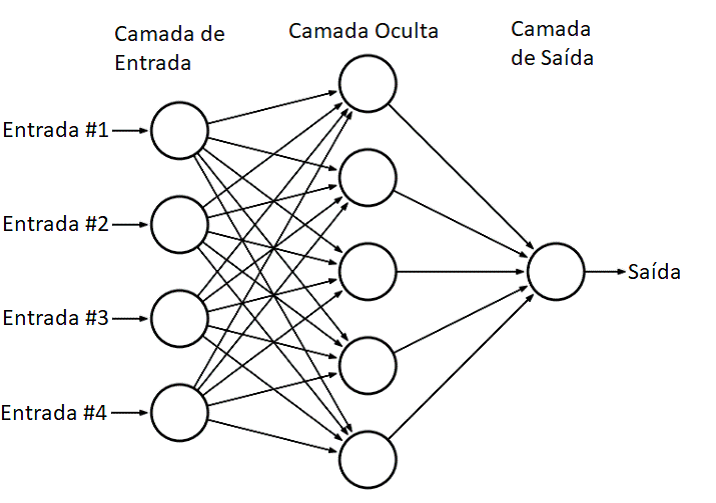
\includegraphics[width=0.6\textwidth]{imagens/arquitetura_mlp.png}
  \caption{Arquitetura MLP. Imagem adaptada de \cite{mlp_architeture_hassan}. \cite{tcc_anomalia_2021}}
  \label{fig:arquitetura_mlp}
  %\legend{Fonte: o autor.}
\end{figure}

A razão pela qual a rede \ac{MLP} resolve o problema do não aprendizado de funções não linearmente separáveis do \textit{perceptron} é a função utilizada nos neurônios. No modelo \textit{perceptron}, tínhamos a função \textit{sign}, que determinava um limiar para a saída ser 1 ou -1. No caso do \ac{MLP}, utiliza-se funções não lineares como função de ativação. E, a conexão de vários \textit{perceptrons} em rede utilizando funções não lineares para o aprendizado é justamente o que possibilita que se aprenda funções não lineares e extremamente complexas. \cite{MLP_gardner}

%%%%%%%%%%%%%%%%%%%%%%%%%%%%%%%%%%%%%%%%%%%%%%
% O que é MLP(CONJ DE PERCEPTRONs conectados, q permitem resolver a limitação do perceptron)
% img arquitetura
% conj d funções não lineares com fç de ativação permite aprender qq parada

\subsection{Função de Ativação}
Como já mencionado anteriormente, a função de ativação consiste em uma das partes da computação do neurônio (ou \textit{perceptron}). A primeira parte é a soma da multiplicação dos dados recebidos com os pesos do neurônio, que então é fornecida como entrada para a função de ativação, que determina a saída do neurônio, consistindo na segunda parte da computação.

Como a maioria dos problemas do mundo real possuem características não lineares, funções de ativação não lineares são preferíveis ao invés de funções lineares.\cite{activation_functions_ann_sharma}. Esse também é o motivo pelo qual funções de ativação são necessárias, já que sem elas, as redes neurais teriam sempre saídas lineares, e agiriam apenas como modelos de regressão linear com desempenho limitado.\cite{tcc_anomalia_2021}

%%%%%%%%%%%%%%%%%%%%%%%%%%%%%%%%%%%%%%%%%%%%%%
% intro opcional sobre oq é a fç de ativação
% Sharma e Athaiya : pq fçs não lineares são necessáriase importantes (2021)
% explicar sigmoid, com fórmula, gráfico. E sua desvantagens
% explicar tanh, com  fórmula, gráfico. E suas desvantagens
% explicar ReLu, com  fórmula, gráfico. E suas desvantagens
% explicar suscintamente LeakyRelu e Parametric ReLu



\subsection{Back Propagation}



\section{Redes Neurais Convolucionais}

\section{Autoencoder}

\section{Classificador}

\begin{comment}
Esse capítulo será responsável por dar uma base teórica a proposta. 
A ideia é que o leitor, com um breve conhecimento prévio, tenha a capacidade de ler esse material e consiga ter a capacidade de entender tecnicamente a proposta do projeto final.
Dependendo do assunto, poderá ter mais de uma área de resumo, podendo ficar cada uma em uma seção ou serem capítulos separados.

No caso de um único capítulo, deverá ter um breve resumo antes de iniciar a seção explicando o que este capítulo fará. Caso seja capítulo separado, poderá introduzir a área diretamente sem a criação de uma seção ou criar uma seção chamada "Introdução" e o nome do capítulo pode ser o nome da área.
\end{comment}
\chapter{Desafios da Detecção de Anomalia }\label{chp:DESAFIOS_DETECCAO_DE_ANOMALIA}

Esse capítulo tem como objetivo promover um maior entendimento sobre o tema Detecção de Anomalia, tratando-o com mais detalhes e explicando suas motivações e desafios. Será abordado também o tema Aprendizado de Máquina, primordial para o entendimento do problema, e seus diversos tipos. E, por último, Redes Neurais, que geralmente é a técnica de aprendizado de máquina utiliza para a identificação de cenários anômalos.

% \section{Detecção de Anomalia}
% O reconhecimento de padrões é muito importante para diversas áreas da ciência. Os objetos a serem classificados podem ser vários, como imagens, formas de onda para aplicação em speech recognition ou produtos em uma fábrica. Hoje em dia, o reconhecimento de padrões é uma parte primordial de vários sistemas de \textit{machine learning} voltados para tomada de decisões.

% \subsection{Desafios da Detecção de Anomalia}
% % dificuldade e achar dataset labeled, desbalanceamento de classe, fortemente dependente do contexto %
% \subsection{Métodos para Detecção de Anomalia}
% %só falar q um classificador não rola devido ao desbalanceamento, q podemos simplesmente treinar %
\section{Desbalanceamento de Classe}

\section{Forte Dependência do Contexto}

\section{Dificuldade em Encontrar Dados Rotulados}

\section{Modelo Utilizado para Detecção de Anomalia}

\begin{comment}
Esse capítulo será responsável por dar uma base teórica a proposta. 
A ideia é que o leitor, com um breve conhecimento prévio, tenha a capacidade de ler esse material e consiga ter a capacidade de entender tecnicamente a proposta do projeto final.
Dependendo do assunto, poderá ter mais de uma área de resumo, podendo ficar cada uma em uma seção ou serem capítulos separados.

No caso de um único capítulo, deverá ter um breve resumo antes de iniciar a seção explicando o que este capítulo fará. Caso seja capítulo separado, poderá introduzir a área diretamente sem a criação de uma seção ou criar uma seção chamada "Introdução" e o nome do capítulo pode ser o nome da área.
\end{comment}
\chapter{Avaliação da Adição de Captions na Detecção de
Anomalia}\label{chp:PROPOSTA}

Esse capítulo será responsável por explicar como será a sua solução.
Ele deverá explicar o problema em que a sua solução irá resolver.
Nele irá conter COMO deverá ser a sua solução, ou seja, neste momento você não está preocupado com a implementação ou ferramentas.
Aqui será relatado o problema e a sua proposta. 
Nela será incluída a modelagem da solução, sua arquitetura e tudo o que for necessário para que o leitor consiga entender COMO será a solução e como ela resolverá o problema relatado.

Além disso, uma parte fundamental, é tratar de trabalhos relacionados. Dependendo da forma de escrita, o trabalho relacionado pode estar explicado no capítulo de Fundamentação ou ser uma seção dentro da proposta antes de entrar na proposta em si.

\section{Introdução}

\section{Trabalhos Relacionados}

\section{Método para avaliação da Adição de Captions na Detecção de Anomalia}

\subsection{Autoencoder Convolucional com MLP}
\subsection{Autoencoder Convolucional}
\subsection{Classificador}


\chapter{Experimentos}\label{chp:EXPERIMENTOS}

Este capítulo falará da solução em execução, ou seja, quais ferramentas escolhidas e seus motivos, como ele foi desenvolvido e como ele atuou em comparação aos trabalhos relacionados.

\section{Base de Dados}

% Falar sobre a escolha de um arquivo, captação de frames, divindo por 3, cerca de 1000 imagens %

\section{Metodologia}
\subsection{OFA}
\subsection{O \textit{framework} Gensim}
\subsection{O \textit{framework} Pytorch}
\subsection{O \textit{framework} ScikitLearn}
\subsection{Validação dos Modelos}
% Flr da divisão dos dados em 3 conjuntos: treino, teste e validação %  
\subsection{Métricas}
\subsection{Arquitetura da Rede Neural Convolucional e Multilayer Perceptron}
\subsection{Arquitetura da Rede Neural Convolucional}
\subsection{Escolha do Limiar de Anomalia}

\section{Resultados}
% 1. tabela com as informações das execuções (quantas forem, as 20, 30, 40, execuções q eu fizer, sei lá)
%  Informações: erro médio para cada classe, f1 score e acurácia para cada modelo. //nem sei se precisa de standard deviation 
 
% 2. tabela com a média das informações da tab anterior (resumo dos resultados) //acho q vai ser tipo uma cópia da tabela lá de cima do capítulo 1, resumo dos resultados

% 3. matrizes de confusão de cada modelo

% 4. É aqui mesmo que vc vai falar da conclusão do experimento, se colocar as captions ajudou ou não na detecção das anomalias. Se sim ou se não, dissertar possíveis motivos.

%%%%%%%%%%%%%%%%%%%%%%%%%%%%%%%%%%%%%%%%%%%%%%%%%%%%%%%%%%%%%%%%%%%%%%%%%
% \section{Métrica de Avaliação}

% \section{Análise dos Experimentos}

% \subsection{Mixed-input}
% \subsection{Classificador Mixed-input}
% \subsection{Convolutional Neural Network}
% \subsection{Classificador Convolutional Neural Network}
% \subsection{Experimento Mixed-input}
% \subsection{Experimento Convolutional Neural Network}

% \section{Resultados}
% \subsection{Experimento Mixed-input}
% \subsection{Experimento Mixed-input}    
\chapter{Conclusão}\label{chp:CONCLUSAO}

Falará um breve resumo do capítulo.

\section{Resumo do Problema Abordado}
\section{Resumo da Proposta}
\section{Resumo dos Resultados}
\section{Principais Contribuições}
\section{Trabalhos Futuros}

% \section{Considerações finais}

% Fará um breve resumo do que foi feito e considerações sobre.

% \section{Limitações e trabalhos futuros}

% Falará sobre as limitações do trabalho e possíveis extensões.

\pagebreak

%%%%%%%%%%%%%%%%%%%%%%%%%%%%%%%%%%%%%%%%%%%%%%%%%%%%%%%%%%%%
% B I B L I O G R A F I A
%%%%%%%%%%%%%%%%%%%%%%%%%%%%%%%%%%%%%%%%%%%%%%%%%%%%%%%%%%%%
% Retirar esta parte se o trabalho não tiver bibliografia
\makebibspage{elementos-postextuais/referencias}

%%%%%%%%%%%%%%%%%%%%%%%%%%%%%%%%%%%%%%%%%%%%%%%%%%%%%%%%%%%%
% A P E N D I C E
%%%%%%%%%%%%%%%%%%%%%%%%%%%%%%%%%%%%%%%%%%%%%%%%%%%%%%%%%%%%
% Retirar esta parte se o trabalho não tiver anexos
\appendix
\chapter{Dicas e Boas Práticas} \label{chp:ap_dicas}

Esse apêndice tem como objetivo explicar como construir um texto científico, apresentando dicas na construção do texto e demonstrando exemplos de códigos em LaTeX para as principais necessidades na elaboração do texto.

% ---
\section{Inclusão de outros arquivos}
% ---

É uma boa prática dividir o seu documento em diversos arquivos, 
e não
apenas escrever tudo em um único. 
Esse recurso foi utilizado neste documento. 
Para incluir diferentes arquivos em um arquivo principal, 
de modo que cada arquivo incluído fique em uma página diferente, utilize o comando:

\begin{verbatim}
   \include{documento-a-ser-incluido}      % sem a extensão .tex
\end{verbatim}

Para incluir documentos sem quebra de páginas, utilize:

\begin{verbatim}
   \input{documento-a-ser-incluido}      % sem a extensão .tex
\end{verbatim}

% ---
\section{Citações}
% ---

AQUI FALAR SOBRE CITACOES

% ---
\section{Imagens e Tabelas}\label{sec:LABEL_CHP_2_SEC_A}
% ---

Toda tabela~\ref{tab:MATRIX_NOTAS_EXEMPLO}

\begin{table}[!htb]
  \centering
  \caption{Fragmento de uma matriz de notas de um sistema de recomendação de filmes.}
  \label{tab:MATRIX_NOTAS_EXEMPLO}
  \rowcolors{1}{}{lightlightgray}
  \begin{tabular}{l c c c}
  \toprule
    & Titanic & Poderoso Chefão & Matrix \\
    \midrule
        Filipe Braida & 4 & $\emptyset$ & 3  \\
        Leandro Alvim & 4 & 5 & 5  \\
        Bruno Dembogurski & 4 & 5 & 5  \\
        Fellipe Duarte & $\emptyset$ & 5 & $\emptyset$  \\ 
    \bottomrule
  \end{tabular}
\end{table}

\section{Images}\label{sec:LABEL_CHP_2_SEC_B}
Reference: \url{http://en.wikibooks.org/wiki/LaTeX/Importing_Graphics}

\begin{figure}
  \centering
  \includegraphics[width=0.6\textwidth]{imagens/chick.png}
  \caption{Chick}
  \label{fig:LABEL_FIG_1}
  \legend{Fonte: o autor.}
\end{figure}

\begin{algorithm}[H]
\floatname{algorithm}{Algoritmo}

\textbf{Entrada} conjunto de notas $R$, limiar $\tau$, modelo de previsão $\varphi$.

\textbf{Saída} conjunto de notas sem ruídos $R^{*}$.

$R^{*} \gets \{\}$

\For{$(u, i, r) \in R$}{
$\tilde{r} \gets \varphi(u,i)$\;

\If{$|\tilde{r} - r| < \tau$}{
$R^{*} \gets R^{*} \cup \{(u,i,r)\}$
}
}
\caption{Filtragem das avaliações com ruído proposto por \cite{OMahony2006}.}
\label{alg:mahony}
\end{algorithm}

\section{Equações}
Reference: \url{http://en.wikibooks.org/wiki/LaTeX/Mathematics}

Also: \url{http://en.wikibooks.org/wiki/LaTeX/Advanced_Mathematics}

\begin{equation}
  (x + y)^2 = x^2 + 2xy + y^2
  \label{eq:LABEL_EQ_1}
\end{equation}

\section{Listings}\label{sec:LABEL_CHP_2_SEC_D}
Reference: \url{http://en.wikibooks.org/wiki/LaTeX/Source_Code_Listings}

\codec{C}{alg:LABEL_CODE_1}{codigos/codigo-c.txt}

\codejava{Java}{alg:LABEL_CODE_2}{codigos/codigo-java.txt}

\section{References}\label{sec:LABEL_CHP_2_SEC_E}

\begin{alineas}
  \item Referencing \refchapter{chp:LABEL_CHP_1}
  \item Referencing \refsection{sec:LABEL_CHP_1_SEC_A}
  \item Referencing \refsection{sec:LABEL_CHP_1_SEC_C}
  \item Referencing \reftable{tab:LABEL_TAB_1}
  \item Referencing \reffigure{fig:LABEL_FIG_1}
  \item Referencing \refequation{eq:LABEL_EQ_1}
  \item Referencing \reflisting{alg:LABEL_CODE_1}
  \item Article \cite{braida2015transforming}
  \item Segundo \citeonline{braida2015transforming}, ....
  \item Referencing \refappendix{chp:LABEL_APP_1}  
\end{alineas}



\section{Definições, Teoremas}

\begin{definition}\label{def:def1}
  Aqui é uma nova definição.
\end{definition}

\begin{definition}[Título] \label{def:def2}
  Aqui é uma outra definição.
\end{definition}

\begin{theorem}\label{the:the1}
  Aqui é um teorema.
\end{theorem}

Seguindo a Definição~\ref{def:def1} e Teorema~\ref{the:the1}.



\section{Acrônimos, Siglas}
  Um \ac{SR}... Portanto, o \ac{SR}...


\section{Símbolos}
  A \ac{rv} é dada por... Assim, \ac{rv}...

\end{document}